\chapter{Results and Discussion}
\label{ch:results}
This chapter presents the experimental results of the proposed Hierarchical Federated Learning framework on the METR-LA dataset. Section~\ref{sec:ablation_results} reports the cumulative ablation study that isolates the contribution of each framework component. Section~\ref{sec:horizon_analysis} analyzes prediction accuracy across different forecast horizons. Section~\ref{sec:cluster_analysis} examines per-cluster performance variations. Section~\ref{sec:lit_comparison} compares the framework against published centralized and federated baselines. Section~\ref{sec:comm_analysis} presents the communication cost analysis. Section~\ref{sec:pemsbay_results} reports cross-dataset validation on PEMS-BAY. Section~\ref{sec:discussion} discusses the key findings, communication--accuracy trade-offs, multi-seed robustness analysis, and limitations.
\section{Ablation Study Results}
\label{sec:ablation_results}
The proposed framework was evaluated through a cumulative ablation study on the METR-LA dataset (207 sensors, 60 communication rounds for the final configuration). Each row in Table~\ref{tab:ablation_results} adds one component to the previous configuration, isolating its individual contribution. For the controlled cumulative ablation, all runs used the same preprocessed data, random seed, and GRU Seq2Seq architecture described in Chapter~\ref{ch:implementation}. Additional multi-seed evaluation for Run~A and Run~G is reported in Section~\ref{sec:multiseed}.

\begin{table}[H]
\centering
\caption{Cumulative ablation study results on METR-LA. Bold indicates the best result in each column. $\Delta$ shows the relative change in MAE compared to the previous row.}
\label{tab:ablation_results}
\small
\begin{tabular}{c l c c c c c}
\hline
\textbf{Run} & \textbf{Configuration} & \textbf{MAE} & \textbf{RMSE} & \textbf{MAPE (\%)} & \textbf{Comm (GB)} & \textbf{$\Delta$ MAE} \\
\hline
A & Global FedAvg & 3.832 & 7.171 & 11.11 & 24.3 & --- \\
B & + DTW Clustering & 3.753 & 7.109 & 10.74 & 24.3 & $-$2.1\% \\
C & + QW + Hier Agg (geo) & 3.722 & 7.093 & 10.51 & 24.5 & $-$0.8\% \\
D & + Adaptive Selection & 3.736 & 7.096 & 10.63 & 21.5 & +0.4\% \\
E & + Time-of-Day Features & 3.700 & 6.841 & 10.74 & 21.5 & $-$1.0\% \\
F & + DTW Hier Weighting & 3.696 & 6.840 & 10.67 & 21.5 & $-$0.1\% \\
G & + LR Decay + $\alpha{=}0.9$ & \textbf{3.676} & \textbf{6.759} & \textbf{10.46} & 25.8 & $-$0.5\% \\
\hline
\multicolumn{2}{l}{\textit{Total improvement (A $\to$ G)}} & \multicolumn{3}{c}{} & & $-$4.1\% \\
\hline
\end{tabular}
\end{table}

\begin{figure}[H]
\centering
\includegraphics[width=0.85\textwidth]{figures/ablation_mae_chart.png}
\caption{Overall MAE across cumulative ablation configurations on METR-LA.}
\label{fig:ablation_mae}
\end{figure}

The ablation study reveals several important findings:
\begin{itemize}
    \item \textbf{DTW Clustering (A $\to$ B):} DTW-based clustering yields the largest individual gain, reducing MAE by 2.1\% (3.832 $\to$ 3.753). This supports the use of temporal-pattern-aware grouping under non-IID traffic distributions.

    \item \textbf{Quality-Weighted and Hierarchical Aggregation (B $\to$ C):} Adding quality-weighted aggregation and hierarchical synchronization provides a further 0.8\% improvement, suggesting that cluster specialization can be combined with limited inter-cluster knowledge sharing.

    \item \textbf{Adaptive Client Selection (C $\to$ D):} Adaptive selection reduces communication by 12.2\% (24.5 $\to$ 21.5 GB), with only a 0.4\% MAE increase. This represents the main communication--accuracy trade-off in the framework.

    \item \textbf{Time-of-Day Features (D $\to$ E):} Time-of-day encodings improve overall MAE by 1.0\% and are especially useful for longer forecast horizons, as discussed in Section~\ref{sec:horizon_analysis}.

    \item \textbf{DTW-Based Hierarchical Weighting (E $\to$ F):} DTW-distance-based inter-cluster weighting gives a marginal 0.1\% improvement. This result is directionally consistent with the proposed design but should not be treated as statistically conclusive.

    \item \textbf{Final Tuning (F $\to$ G):} Learning-rate decay and stronger cluster specialization ($\alpha=0.9$) provide a small additional improvement, reaching the best controlled seed-42 MAE of 3.676.
\end{itemize}

\section{Prediction Horizon Analysis}
\label{sec:horizon_analysis}
Table~\ref{tab:horizon_results} reports MAE disaggregated by prediction horizon (15, 30, and 60 minutes) for all ablation configurations.
\begin{table}[H]
\centering
\caption{Per-horizon MAE (mph) across ablation configurations on METR-LA.}
\label{tab:horizon_results}
\small
\begin{tabular}{c l c c c c}
\hline
\textbf{Run} & \textbf{Configuration} & \textbf{15 min} & \textbf{30 min} & \textbf{60 min} & \textbf{Overall} \\
\hline
A & Global FedAvg & 3.088 & 3.840 & 4.896 & 3.832 \\
B & + DTW Clustering & 3.015 & 3.755 & 4.805 & 3.753 \\
C & + QW + Hier Agg (geo) & 2.986 & 3.723 & 4.754 & 3.722 \\
D & + Adaptive Selection & 3.002 & 3.735 & 4.780 & 3.736 \\
E & + Time-of-Day Features & 3.074 & 3.739 & 4.565 & 3.700 \\
F & + DTW Hier Weighting & 3.083 & 3.734 & 4.543 & 3.696 \\
G & + LR Decay + $\alpha{=}0.9$ & \textbf{3.051} & \textbf{3.705} & \textbf{4.559} & \textbf{3.676} \\
\hline
\end{tabular}
\end{table}
Two observations stand out from the horizon analysis:
\begin{itemize}
    \item \textbf{Time-of-day features disproportionately improve long-horizon predictions.} Comparing Run~D (speed-only) with Run~E (speed + ToD), the 60-minute MAE improves by 4.5\% (4.780 $\to$ 4.565) while the 15-minute MAE slightly increases (3.002 $\to$ 3.074). This is expected: short-term predictions depend primarily on recent speed values, while longer-horizon forecasts benefit from contextual information about the time of day (e.g., morning peak vs.\ late-night).
    
    \item \textbf{Prediction quality degrades with horizon length.} Across all configurations, the 60-minute MAE is approximately 40--50\% higher than the 15-minute MAE. For the final configuration~G, the ratio is $4.559 / 3.051 = 1.49$, indicating that one-hour predictions are 49\% less accurate than 15-minute predictions. This degradation pattern is consistent with all published traffic forecasting methods on METR-LA \cite{li2018, wu2019graphwavenet}.
\end{itemize}


\clearpage
\section{Per-Cluster Performance Analysis}
\label{sec:cluster_analysis}
Table~\ref{tab:cluster_results} shows the per-cluster MAE breakdown for the final configuration (Run~G, 60 rounds). The eight clusters exhibit substantial performance variation, reflecting the heterogeneous nature of the METR-LA sensor network.

\begin{table}[H]
\centering
\caption{Per-cluster performance breakdown (Run~G, 60 rounds). Clusters are ordered by DTW-based grouping.}
\label{tab:cluster_results}
\begin{tabular}{c r r r}
\hline
\textbf{Cluster} & \textbf{Sensors} & \textbf{MAE (mph)} & \textbf{60 min MAE} \\
\hline
0 & 31 & 3.779 & 4.503 \\
1 & 32 & 3.835 & 4.850 \\
2 & 8 & 2.414 & 2.550 \\
3 & 36 & 4.281 & 5.494 \\
4 & 8 & 2.588 & 3.162 \\
5 & 25 & 4.161 & 5.251 \\
6 & 39 & \textbf{2.000} & \textbf{2.246} \\
7 & 28 & 5.177 & 6.663 \\
\hline
\textit{Overall} & \textit{207} & \textit{3.676} & \textit{4.559} \\
\hline
\end{tabular}
\end{table}

\begin{figure}[H]
\centering
\includegraphics[width=0.78\textwidth]{figures/per_cluster_mae.png}
\caption{Per-cluster MAE for the final configuration on METR-LA. The variation across clusters shows that different DTW-based groups have different levels of prediction difficulty.}
\label{fig:per_cluster_mae}
\end{figure}


The cluster-level results reveal a wide MAE range from 2.000 (Cluster~6) to 5.177 (Cluster~7), a ratio of approximately $2.6\times$. Several factors contribute to this variation:
\begin{itemize}
    \item \textbf{Cluster~6 (39 sensors, MAE = 2.000)} appears to contain sensors with highly regular and low-variability speed profiles, making them easier to forecast. The consistently low MAE across both short and long horizons suggests that sensors in this cluster share stable, predictable temporal patterns.
    \item \textbf{Cluster~7 (28 sensors, MAE = 5.177)} appears to capture more irregular or heterogeneous temporal patterns, which leads to higher forecast error. The large gap between overall and 60-minute MAE (5.177 vs.\ 6.663) suggests that this cluster contains sensors where traffic conditions are difficult to predict at longer horizons.
    \item \textbf{Clusters~2 and 4 (8 sensors each, MAE $\approx$ 2.4--2.6)} are small, highly homogeneous clusters where DTW clustering groups sensors with very similar temporal profiles. The low intra-cluster non-IID divergence allows the cluster model to specialize effectively.
    \item \textbf{Clusters~3 and 5 (36 and 25 sensors, MAE $\approx$ 4.2--4.3)} are larger clusters with moderate internal heterogeneity. Their higher MAE reflects the challenge of fitting a single model to a broader range of traffic patterns within the cluster.
\end{itemize}
These results suggest that DTW-based clustering produces groups with distinct levels of predictive difficulty, reflecting differences in temporal regularity and traffic variability across the sensor network.

\section{Empirical Evidence of Non-IID Sensor Distributions}
\label{sec:noniid_evidence}

A central assumption of this thesis is that traffic sensor data are non-IID. To support this assumption empirically, additional diagnostic analysis was conducted on the raw, pre-normalized METR-LA speed readings. The results show heterogeneity at three levels: distributional differences, temporal-dependence differences, and clustering structure.

First, the marginal speed distributions differ substantially across sensors. Per-sensor mean speeds range from 30.89~mph to 67.73~mph, while per-sensor standard deviations range from 1.90~mph to 23.17~mph. The coefficient of variation ranges from 0.028 to 0.558, indicating that some sensors observe stable high-speed traffic while others experience much more variable traffic behavior. Figure~\ref{fig:noniid_distributions} visualizes these differences across all 207 sensors.

\begin{figure}[H]
\centering
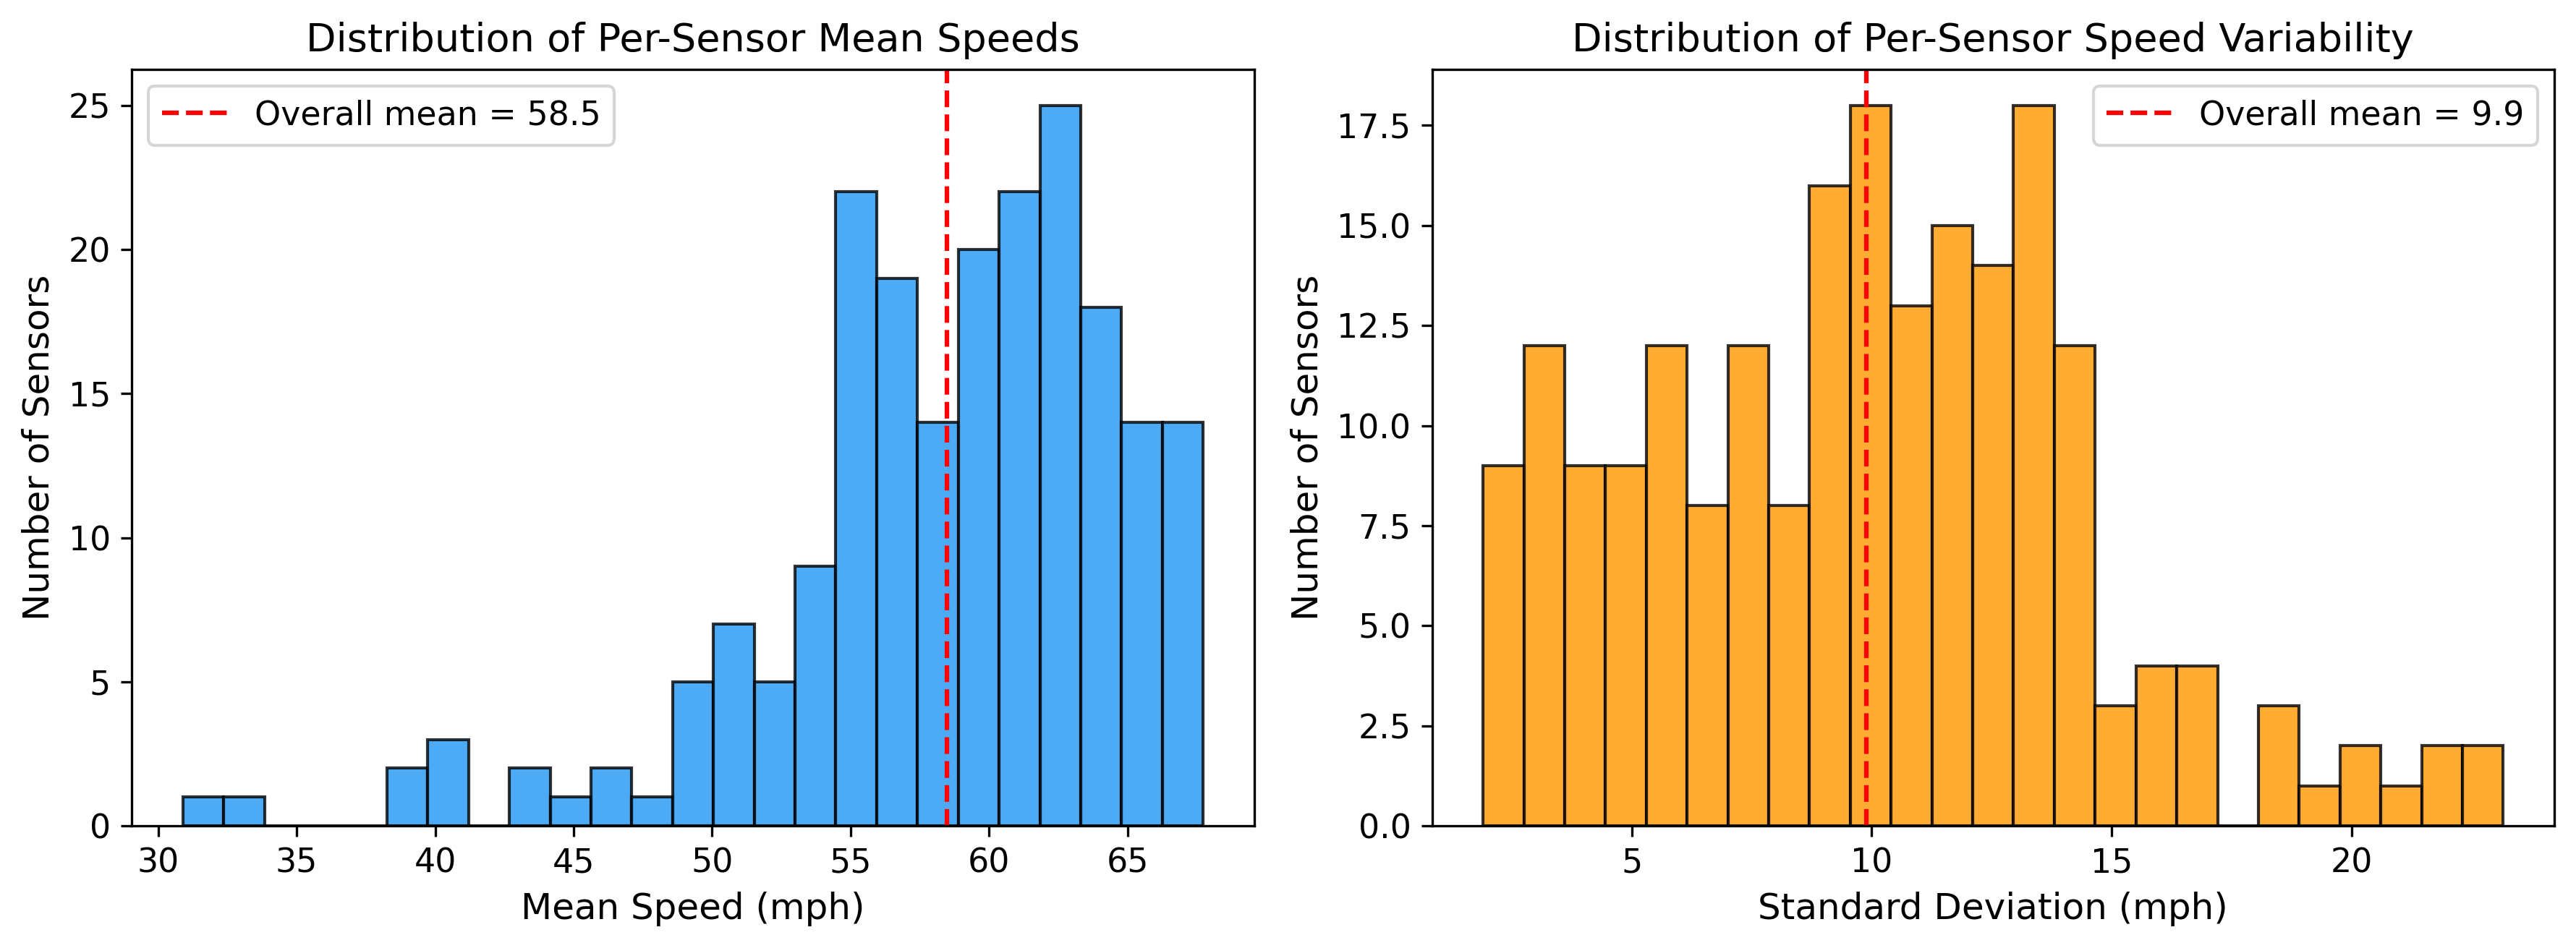
\includegraphics[width=0.9\textwidth]{figures/noniid_sensor_distributions.png}
\caption{Distribution of per-sensor mean speeds and standard deviations across the 207 METR-LA sensors. The wide ranges indicate substantial distribution-level heterogeneity.}
\label{fig:noniid_distributions}
\end{figure}

Second, the temporal structure also differs across sensors. Table~\ref{tab:noniid_summary} shows that traffic speed is strongly autocorrelated, with a mean ACF of 0.838 at lag~1 and 0.522 at lag~12. This confirms that traffic forecasting is a valid time-series prediction problem. However, the large min--max ranges show that the strength of temporal dependence varies considerably across sensors. For example, the one-hour autocorrelation ranges from 0.102 to 0.776, meaning that some sensors retain strong temporal memory while others change more rapidly.

\begin{table}[H]
\centering
\caption{Summary of non-IID diagnostic evidence on METR-LA.}
\label{tab:noniid_summary}
\small
\renewcommand{\arraystretch}{1.15}
\begin{tabular}{p{0.58\textwidth} p{0.28\textwidth}}
\hline
\textbf{Diagnostic} & \textbf{Result} \\
\hline
Per-sensor mean speed range & 30.89--67.73 mph \\
Per-sensor standard deviation range & 1.90--23.17 mph \\
Coefficient of variation range & 0.028--0.558 \\
Mean ACF at lag 1 (5 min) & 0.838 \\
Mean ACF at lag 12 (1 hour) & 0.522 \\
ACF lag 12 range & 0.102--0.776 \\
Mean ACF at lag 288 (1 day) & 0.402 \\
Within/between temporal-distance ratio & 0.913 \\
Permutation test against random clusters & $p < 0.001$ \\
Per-cluster MAE range in Run G & 2.000--5.177 mph \\
\hline
\end{tabular}
\end{table}

Finally, the clustering structure was evaluated by comparing within-cluster and between-cluster distances using z-score normalized 300-step representative series. The mean within-cluster distance was 20.40, compared with 22.34 between clusters, giving a within/between ratio of 0.913. Since this value is below 1.0, sensors within the same cluster are more similar to each other than to sensors in other clusters. A permutation test with 1{,}000 random cluster assignments produced a random ratio of $1.000 \pm 0.005$, with $p < 0.001$. This confirms that the clustering captures statistically significant temporal-pattern structure rather than random grouping.

\begin{figure}[htbp]
\centering
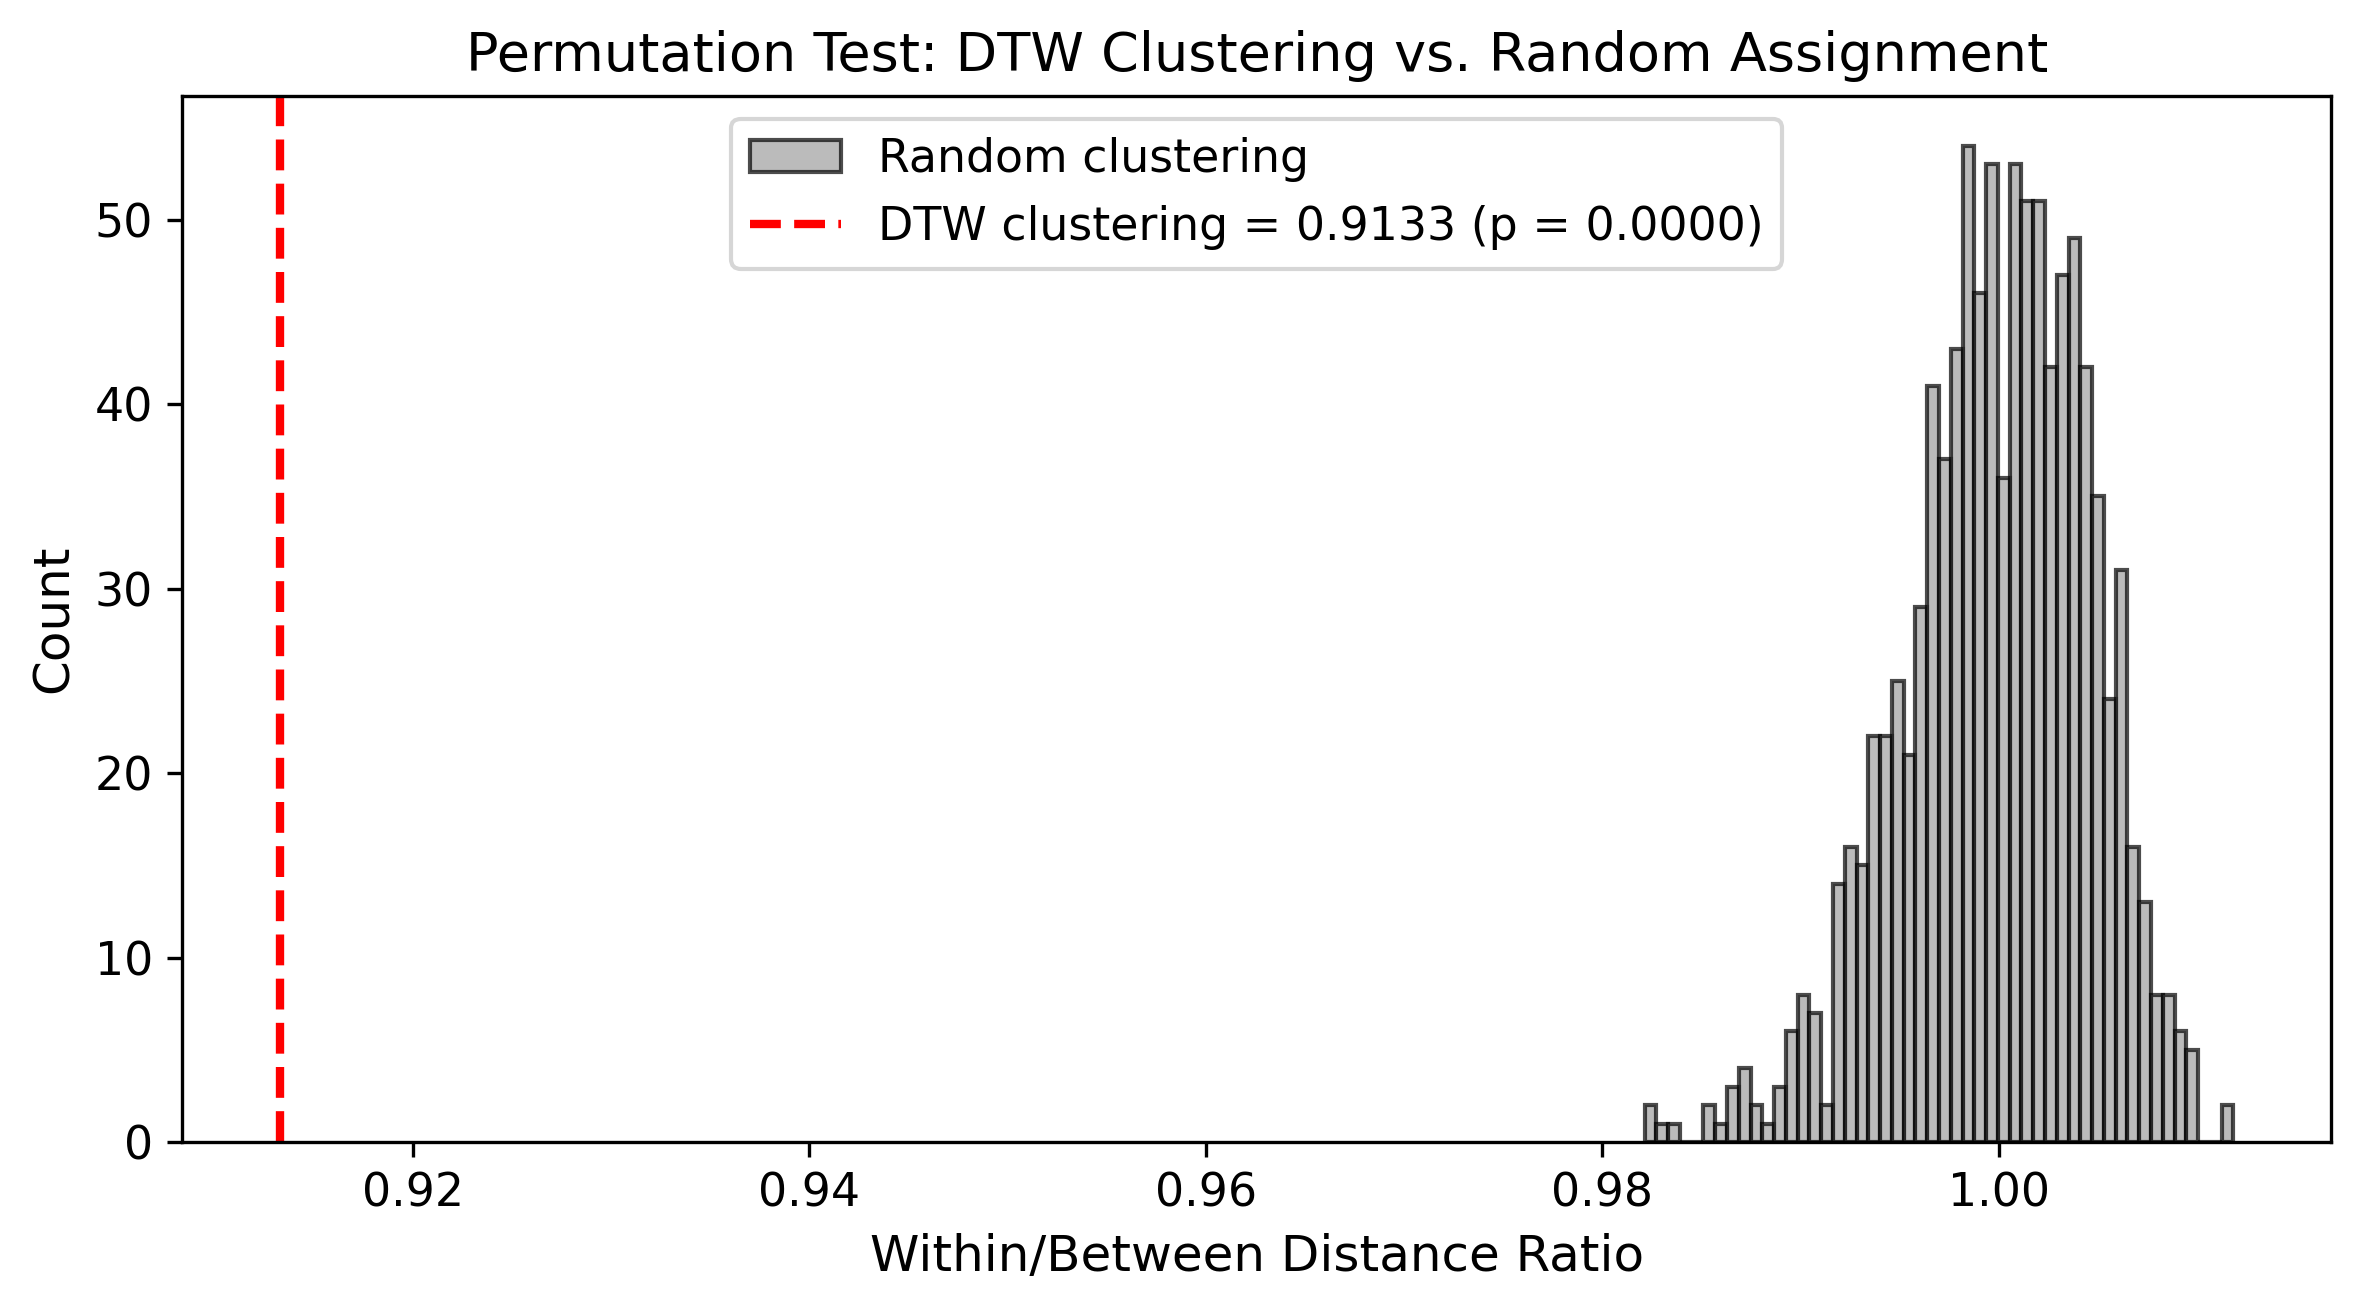
\includegraphics[width=0.75\textwidth]{figures/noniid_permutation_test.png}
\caption{Permutation test comparing the observed within/between temporal-distance ratio against random cluster assignments. The observed ratio is significantly lower than the random baseline ($p < 0.001$).}
\label{fig:permutation_test}
\end{figure}

These diagnostics support the non-IID assumption used throughout the thesis. The METR-LA sensors differ not only in average speed and variability, but also in temporal autocorrelation and prediction difficulty. This justifies the use of clustered federated learning instead of forcing all sensors into a single homogeneous global model.

\section{Statistical and Linear Baselines}
\label{sec:stat_baselines}

To contextualize the proposed framework's accuracy, three simple baselines were evaluated on the same METR-LA test set using identical metrics and denormalization:

\begin{itemize}
    \item \textbf{Persistence (Last Value):} Predicts the last observed speed value for all 12 future horizons. This is the simplest possible time-series baseline.
    \item \textbf{Per-Sensor Historical Mean:} Predicts the per-sensor average speed computed from all training targets. This tests whether the model learns anything beyond the unconditional mean.
    \item \textbf{Ridge Regression ($\alpha = 1.0$):} Fits a per-sensor linear mapping from the 12 input time steps to the 12 output horizons. This directly tests whether a linear model suffices.
\end{itemize}

\begin{table}[H]
\centering
\caption{Comparison with simple statistical and linear baselines on METR-LA.}
\label{tab:statistical_baselines}
\small
\begin{tabular}{lrrrrrr}
\hline
\textbf{Method} & \textbf{MAE} & \textbf{RMSE} & \textbf{MAPE (\%)} & \textbf{15 min} & \textbf{30 min} & \textbf{60 min} \\
\hline
Persistence & 3.854 & 7.800 & 9.74 & 3.160 & 3.828 & 4.902 \\
Per-Sensor Historical Mean & 6.634 & 11.187 & 21.28 & 6.634 & 6.634 & 6.635 \\
Ridge Regression & 3.732 & 7.072 & 10.45 & \textbf{2.996} & 3.720 & 4.793 \\
Global FedAvg (Run A) & 3.832 & 7.171 & 11.11 & 3.078 & 3.868 & 4.896 \\
Proposed HFL (Run G) & \textbf{3.676} & \textbf{6.759} & 10.46 & 3.051 & \textbf{3.705} & \textbf{4.559} \\
\hline
\end{tabular}
\end{table}

Table~\ref{tab:statistical_baselines} shows that simple baselines are highly competitive on METR-LA, which is expected given the strong autocorrelation observed in Section~\ref{sec:noniid_evidence}. The persistence baseline already achieves an overall MAE of 3.854, close to the Global FedAvg baseline. This indicates that recent speed values contain substantial predictive information and confirms the importance of including simple time-series baselines.

Ridge regression further improves over persistence, achieving an overall MAE of 3.732 and the best 15-minute MAE of 2.996. This shows that a linear model can capture a large part of the short-term traffic dynamics. However, the proposed HFL framework achieves the best overall MAE and the best long-horizon performance. Compared with Ridge regression, Run~G reduces overall MAE from 3.732 to 3.676 and reduces 60-minute MAE from 4.793 to 4.559. This corresponds to an approximately 1.5\% overall MAE improvement and a 4.9\% improvement at the 60-minute horizon.

These results refine the motivation for using the GRU Seq2Seq model. The purpose of the recurrent backbone is not to claim that linear models are ineffective; rather, it provides better long-horizon forecasting under the proposed federated framework while maintaining a small model size suitable for repeated FL communication. The strength of the Ridge baseline also confirms that future work should evaluate even lighter linear or hybrid local models within the same hierarchical FL framework.

\section{Comparison with Published Baselines}
\label{sec:lit_comparison}
% Table~\ref{tab:lit_comparison} compares the final framework configuration (Run~G) against published centralized and federated baselines on METR-LA. 

\begin{table}[H]
\centering
\caption{Comparison with published baselines on METR-LA. Communication cost is reported where available.}
\label{tab:lit_comparison}
\small
\begin{tabular}{l l c c c c}
\hline
\textbf{Method} & \textbf{Type} & \textbf{MAE} & \textbf{RMSE} & \textbf{MAPE (\%)} & \textbf{Comm (GB)} \\
\hline
\multicolumn{6}{l}{\textit{Centralized baselines}} \\
\hline
FC-LSTM \cite{hochreiter1997} & Centralized & 4.37 & 8.60 & 13.20 & --- \\
STGCN \cite{yu2018stgcn} & Cent.+Graph & 4.59 & 9.40 & 12.70 & --- \\
\hline
\multicolumn{6}{l}{\textit{Centralized graph-based baselines}} \\
\hline
DCRNN \cite{li2018} & Cent.+Graph & 3.17 & 6.45 & 8.80 & --- \\
Graph WaveNet \cite{wu2019graphwavenet} & Cent.+Graph & 3.07 & 6.22 & 8.40 & --- \\
ASTGCN \cite{guo2019} & Cent.+Graph & 3.38 & 7.10 & --- & --- \\
\hline
\multicolumn{6}{l}{\textit{Federated baselines$\dagger$}} \\
\hline
FedGRU \cite{liu2020fedgru} & Federated & 5.64 & 13.57 & --- & 27.3 \\
CMBA-FL \cite{zhu2025cmba} & Federated & 4.25 & 10.96 & --- & 36.4 \\
\hline
\multicolumn{6}{l}{\textit{Proposed framework}} \\
\hline
\textbf{Ours (Run G)} & \textbf{HFL} & \textbf{3.676} & \textbf{6.759} & \textbf{10.46} & \textbf{25.8} \\
\hline
\end{tabular}
\end{table}

\begin{figure}[H]
\centering
\includegraphics[width=\textwidth]{figures/metr_la_proposed_framework_vs_baselines.png}
\caption{MAE comparison of the proposed framework with published METR-LA baselines. Centralized graph-based methods are shown as contextual upper-bound references because they use full data access and graph structure. Lower MAE indicates better performance.}
\label{fig:metr_la_proposed_framework_vs_baselines}
\end{figure}

% The proposed framework achieves the following results relative to published baselines:
% \begin{itemize}
%     \item \textbf{vs.\ reported centralized baselines:} The framework outperforms both FC-LSTM (MAE 4.37, $-$15.9\%) and STGCN (MAE 4.59, $-$19.9\%) despite operating under federated data isolation. These baselines use centralized data access and, in the case of STGCN, graph structure information.
%     \item \textbf{vs.\ CMBA-FL:} The proposed framework reduces MAE by 13.5\% (4.25 $\to$ 3.676) while using 29.1\% less communication (36.4 $\to$ 25.8~GB). This is a substantial improvement over the most directly comparable federated baseline, which also uses a GRU-based architecture without graph structure.
%     \item \textbf{vs.\ FedGRU:} The proposed framework achieves a 34.8\% lower MAE (5.64 $\to$ 3.676) with 5.5\% less communication (27.3 $\to$ 25.8~GB). The large accuracy gap suggests that naive federated averaging without clustering, quality weighting, or hierarchical aggregation is insufficient for non-IID traffic data.
%     \item \textbf{vs.\ Centralized graph-based models:} The proposed framework achieves an MAE of 3.676, which is within 16.0\% of DCRNN (3.17) and 19.7\% of Graph WaveNet (3.07). Importantly, centralized models assume access to the full sensor network data and graph adjacency structure, while the proposed framework avoids centralizing raw sensor data and operates without any graph structure information. The RMSE of 6.759 is comparable to DCRNN (6.45) and better than ASTGCN (7.10), indicating competitive prediction distribution despite the federated constraint.
% \end{itemize}
The proposed framework outperforms the reported non-graph centralized baseline FC-LSTM and the federated baselines FedGRU and CMBA-FL. Compared with CMBA-FL, the most directly comparable federated baseline, the proposed framework reduces MAE from 4.25 to 3.676 while also reducing communication from 36.4 GB to 25.8 GB. Compared with FedGRU, the framework achieves substantially lower MAE, indicating that naive recurrent FedAvg is insufficient under non-IID traffic distributions.
 
It should be noted that centralized graph-based baselines (DCRNN, Graph WaveNet, ASTGCN) are not directly comparable to the proposed federated setting. They use full centralized data access and explicit spatial graph convolutions, which are unavailable under federated data isolation constraints. These results are therefore presented as contextual upper-bound references rather than direct comparisons.

\section{Communication Cost Analysis}
\label{sec:comm_analysis}
Communication efficiency is a central objective of this thesis. Throughout this work, the term \textit{communication-efficient} is used in the federated-training sense: it refers to reducing repeated model-update communication compared with other FL configurations and published FL baselines. It does not mean that FL transmits fewer bytes than a one-time centralized upload of the historical scalar dataset. For reference, the raw METR-LA speed matrix contains 207 sensors over 34{,}272 time steps and requires approximately 28.4~MB when stored as 32-bit floating-point values. In contrast, FL communication accumulates over many rounds because model parameters are repeatedly exchanged.

Table~\ref{tab:raw_vs_fl_comm} clarifies this distinction. The value of FL in this thesis is therefore not raw byte reduction compared with centralized data upload, but distributed training under data locality, governance, and edge-deployment constraints.

\begin{table}[htbp]
\centering
\caption{Comparison between one-time raw-data size and repeated FL model communication on METR-LA.}
\label{tab:raw_vs_fl_comm}
\begin{tabular}{l l l}
\hline
\textbf{Quantity} & \textbf{Approx.\ Size} & \textbf{Interpretation} \\
\hline
One-time METR-LA speed matrix (float32) & 28.4 MB & Centralized historical upload \\
DTW initialization overhead & 0.25 MB & One-time clustering setup \\
Single model transfer & 1.26 MB & Per-client per-round \\
Run F FL communication & 21.5 GB & Comm-efficient operating point \\
Run G FL communication & 25.8 GB & Best-accuracy operating point \\
CMBA-FL FL communication & 36.4 GB & Published FL baseline \\
\hline
\end{tabular}
\end{table}

Reported communication costs are converted from logged megabytes using a 1024~MB per GB convention. Table~\ref{tab:comm_analysis} reports the communication cost for each ablation configuration.

\begin{table}[htbp]
\centering
\caption{Communication cost across ablation configurations.}
\label{tab:comm_analysis}
\begin{tabular}{c l r r r}
\hline
\textbf{Run} & \textbf{Configuration} & \textbf{Comm (GB)} & \textbf{Participation} & \textbf{Rounds} \\
\hline
A & Global FedAvg & 24.3 & 100\% & 50 \\
B & + DTW Clustering & 24.3 & 100\% & 50 \\
C & + QW + Hier Agg & 24.5 & 100\% & 50 \\
D & + Adaptive Selection & 21.5 & 75\% & 50 \\
E & + Time-of-Day Features & 21.5 & 75\% & 50 \\
F & + DTW Hier Weighting & 21.5 & 75\% & 50 \\
G & + LR Decay + $\alpha{=}0.9$ & 25.8 & 75\% & 60 \\
\hline
\end{tabular}
\end{table}

\begin{figure}[H]
\centering
\includegraphics[width=0.78\textwidth]{figures/communication_cost_ablation.png}
\caption{Communication cost across ablation configurations on METR-LA. Adaptive client selection reduces communication from Run C to Run D, while Run G increases total communication because it uses additional training rounds.}
\label{fig:communication_cost_ablation}
\end{figure}


The results show two main trends. First, adaptive client selection reduces communication from 24.5~GB in Run~C to 21.5~GB in Run~D, a 12.2% reduction at the same number of communication rounds. This reduction comes mainly from fewer client uploads per round, while cluster-model broadcasts to all members remain unchanged. Second, the best-accuracy configuration, Run~G, increases total communication to 25.8~GB because it uses 60 rounds instead of 50. This additional communication improves MAE from 3.696 in Run~F to 3.676 in Run~G.

The proposed framework should therefore be interpreted as offering two operating points. Run~F is the communication-efficient configuration, achieving MAE~=~3.696 with 21.5~GB of communication. Run~G is the best-accuracy configuration, achieving MAE~=~3.676 with 25.8~GB of communication. Compared with CMBA-FL, which requires 36.4~GB and reports MAE~=~4.25 \cite{zhu2025cmba}, Run~G reduces communication by 29.1% while improving MAE by 13.5%.

It should also be noted that Run~G uses slightly more total communication than Global FedAvg, because it uses 60 rounds and includes hierarchical synchronization overhead. Therefore, the communication savings of the proposed framework are most accurately characterized as a reduction relative to published FL baselines and as a per-round upload reduction through adaptive client selection, rather than an absolute reduction across all operating points.

\section{Cross-Dataset Validation: PEMS-BAY}
\label{sec:pemsbay_results}

To assess generalization beyond METR-LA, the final framework configuration was evaluated on the PEMS-BAY dataset (325 sensors). Due to computational budget constraints, the PEMS-BAY experiment was limited to 50 communication rounds rather than the 60 used for the final METR-LA configuration. Table~\ref{tab:pemsbay_results} compares the proposed framework against published baselines on PEMS-BAY, with baseline results taken from Zhu et al. \cite{zhu2025cmba}.

\begin{table}[H]
\centering
\caption{Cross-dataset validation on PEMS-BAY. Published baseline results are from Zhu et al. \cite{zhu2025cmba}. Communication costs are reported where available.}
\label{tab:pemsbay_results}
\small
\setlength{\tabcolsep}{4pt}
\renewcommand{\arraystretch}{1.15}
\begin{tabular}{l l c c c c}
\hline
\textbf{Method} & \textbf{Setting} & \textbf{MAE} & \textbf{RMSE} & \textbf{MAPE (\%)} & \textbf{Comm (GB)} \\
\hline
\multicolumn{6}{l}{\textit{Centralized baselines (reported)}} \\
\hline
FC-LSTM \cite{hochreiter1997} & Centralized & 2.37 & 4.96 & 5.70 & --- \\
STGCN \cite{yu2018stgcn} & Cent.+Graph & 2.49 & 5.69 & 5.79 & --- \\
\hline
\multicolumn{6}{l}{\textit{Federated baselines (reported)}} \\
\hline
FedGRU \cite{liu2020fedgru} & Federated & 2.23 & 4.85 & 5.52 & 38.3 \\
CMBA-FL \cite{zhu2025cmba} & Federated & \textbf{1.72} & \textbf{3.80} & \textbf{4.00} & 48.1 \\
\hline
\multicolumn{6}{l}{\textit{Proposed framework}} \\
\hline
\textbf{Ours (Run G)} & \textbf{HFL} & 2.052 & 4.366 & 4.93 & \textbf{33.6} \\
\hline
\end{tabular}
\end{table}

\begin{figure}[H]
\centering
\includegraphics[width=\textwidth]{figures/pemsbay_proposed_framework_vs_baselines.png}
\caption{MAE comparison of the proposed framework with published PEMS-BAY baselines. CMBA-FL achieves the lowest MAE, while the proposed framework provides lower communication cost. Lower MAE indicates better performance.}
\label{fig:pemsbay_proposed_framework_vs_baselines}
\end{figure}

The framework achieves an overall MAE of 2.052 on PEMS-BAY. This value is lower than the METR-LA result of 3.676, which is consistent with the commonly observed lower prediction difficulty of PEMS-BAY compared with METR-LA~\cite{li2018}, as PEMS-BAY generally exhibits more regular freeway traffic patterns. The per-horizon breakdown is: 15~min MAE = 1.570, 30~min MAE = 2.088, 60~min MAE = 2.723.

% The proposed framework's PEMS-BAY results support the following observations:

% \begin{itemize}
%     \item The framework outperforms the reported centralized baselines FC-LSTM (MAE 2.37, $-$13.4\%) and STGCN (MAE 2.49, $-$17.6\%), as well as the federated baseline FedGRU (MAE 2.23, $-$8.0\%).

%     \item CMBA-FL achieves better accuracy (MAE 1.72) on PEMS-BAY, but at a substantially higher communication cost of 48.1~GB compared with 33.6~GB for the proposed framework, a 30.1\% communication reduction. This mirrors the METR-LA comparison in terms of communication efficiency, although unlike METR-LA, CMBA-FL remains more accurate on PEMS-BAY.

%     \item The PEMS-BAY experiment was limited to 50 communication rounds due to computational budget constraints, compared with 60 rounds for METR-LA. The convergence analysis in Section~\ref{sec:convergence} suggests that additional rounds with learning rate scheduling could further reduce the MAE gap relative to CMBA-FL.

%     \item The same core framework configuration---DTW clustering with $K=8$, quality-weighted hierarchical aggregation, adaptive client selection, and time-of-day features---was applied without dataset-specific architectural modifications, providing preliminary evidence that the framework can transfer across sensor networks, although further dataset-specific tuning and additional training rounds would be needed for a stronger generalization claim.
% \end{itemize}

The PEMS-BAY results show that the same framework can be applied to a different sensor network without dataset-specific architectural changes. The proposed framework outperforms FC-LSTM, STGCN, and FedGRU, but CMBA-FL remains more accurate on this dataset. However, the proposed framework uses 30.1\% less communication than CMBA-FL (33.6 GB vs. 48.1 GB), showing that the main advantage on PEMS-BAY is communication efficiency rather than absolute accuracy. Because the PEMS-BAY experiment was limited to 50 rounds and one seed, this result should be interpreted as preliminary cross-dataset validation rather than conclusive generalization evidence.
\clearpage
\section{Discussion}
\label{sec:discussion}
\subsection{Key Findings}

The results highlight five main findings. First, DTW-based clustering is the largest individual contributor to accuracy improvement in the controlled ablation. Second, quality-weighted hierarchical aggregation improves performance in the seed-42 ablation, suggesting that cluster specialization can be combined with limited inter-cluster knowledge sharing. Third, adaptive client selection creates a deliberate communication--accuracy trade-off by reducing upload communication while causing only a small MAE increase. Fourth, time-of-day features mainly benefit longer forecast horizons. Finally, the PEMS-BAY experiment provides preliminary evidence of cross-dataset transfer, although CMBA-FL remains more accurate on that dataset.

\subsection{Communication--Accuracy Trade-off}
The results reveal two practical operating points for the proposed framework. Run~F provides the most communication-efficient configuration, achieving MAE = 3.696 with 21.5~GB total communication over 50 rounds. Run~G provides the highest-accuracy configuration, reducing MAE to 3.676 at the cost of increased communication (25.8~GB) due to 10 additional training rounds. This illustrates that the proposed framework can be tuned depending on whether the deployment prioritizes lower communication cost or maximum forecasting accuracy.
Both operating points outperform CMBA-FL (MAE = 4.25, 36.4~GB) in both accuracy and communication. Even the communication-efficient Run~F achieves 13.0\% better MAE than CMBA-FL while using 40.9\% less communication. This suggests that the proposed hierarchical approach offers a favorable accuracy--communication frontier compared to existing federated traffic forecasting methods.

\subsection{Convergence Behavior Before Final Tuning}
\label{sec:convergence}
The training convergence before final learning-rate tuning was analyzed using intermediate evaluation metrics recorded every five rounds for Run~F. Figure~\ref{fig:convergence_run_f} shows the trajectory for Run~F, the 50-round DTW-weighted hierarchical configuration. This run is useful for assessing whether additional rounds alone improve performance before introducing the learning-rate schedule used in Run~G.
% \begin{table}[H]
% \centering
% \caption{Convergence trajectory for Run~F (50 rounds).}
% \label{tab:convergence}
% \begin{tabular}{r c c c}
% \hline
% \textbf{Round} & \textbf{MAE} & \textbf{60 min MAE} & \textbf{Avg Loss} \\
% \hline
% 5 & 3.921 & 4.915 & 0.502 \\
% 10 & 3.847 & 4.833 & 0.508 \\
% 15 & 3.834 & 4.798 & 0.481 \\
% 20 & 3.811 & 4.744 & 0.487 \\
% 25 & 3.797 & 4.695 & 0.474 \\
% 30 & 3.748 & 4.625 & 0.460 \\
% 35 & 3.747 & 4.623 & 0.448 \\
% 40 & 3.716 & 4.582 & 0.439 \\
% 45 & 3.708 & 4.555 & 0.428 \\
% 50 & 3.696 & 4.543 & 0.440 \\
% \hline
% \end{tabular}
% \end{table}
\begin{figure}[H]
\centering
\includegraphics[width=0.78\textwidth]{figures/convergence_run_f.png}
\caption{Convergence trajectory of Run F over 50 communication rounds. The overall MAE and 60-minute MAE improve steadily, but the rate of improvement slows in later rounds, motivating the learning-rate schedule used in Run G.}
\label{fig:convergence_run_f}
\end{figure}

The convergence trajectory shows steady improvement throughout training, with MAE decreasing from 3.921 at round~5 to 3.696 at round~50. The rate of improvement slows in later rounds (0.012 MAE improvement from round~45 to~50 vs.\ 0.074 from round~5 to~10), indicating that the model approaches convergence by round~50. An extended 75-round experiment with the same configuration achieved MAE = 3.697 at round~75, confirming that additional rounds beyond 50 provide minimal benefit without learning rate scheduling. This supports the decision to use learning rate decay (Run~G) rather than simply increasing the number of rounds.

\subsection{Multi-Seed Robustness Analysis}
\label{sec:multiseed}
The cumulative ablation study uses a single random seed (42) to ensure a controlled comparison across configurations. To verify that the overall improvement of the proposed framework is not an artifact of a particular random initialization, the two most critical configurations---Run~A (Global FedAvg baseline) and Run~G (final proposed framework)---were evaluated with three independent random seeds (42, 123, 456). The random seed controls model weight initialization, client reliability profile assignment, and per-round client availability sampling.

Table~\ref{tab:multiseed} reports the per-seed and aggregated results. Note that the cumulative ablation table (Table~\ref{tab:ablation_results}) and baseline comparison tables report the controlled seed-42 run used for component-wise comparison (MAE = 3.676), while this section reports the mean performance across seeds (MAE = $3.620 \pm 0.049$).

\begin{table}[H]
\centering
\caption{Multi-seed evaluation of Run~A (Global FedAvg) and Run~G (proposed framework) on METR-LA. Three seeds vary weight initialization and client selection randomness.}
\label{tab:multiseed}
\small
\begin{tabular}{l c c c c}
\hline
\textbf{Seed} & \textbf{MAE} & \textbf{RMSE} & \textbf{MAPE (\%)} & \textbf{60 min MAE} \\
\hline
\multicolumn{5}{l}{\textit{Run A --- Global FedAvg}} \\
\hline
42  & 3.832 & 7.171 & 11.11 & 4.896 \\
123 & 3.825 & 7.046 & 11.43 & 4.694 \\
456 & 3.853 & 7.091 & 11.64 & 4.722 \\
\textit{Mean $\pm$ std} & \textit{3.837 $\pm$ 0.015} & \textit{7.103 $\pm$ 0.063} & \textit{11.39 $\pm$ 0.27} & \textit{4.771 $\pm$ 0.109} \\
\hline
\multicolumn{5}{l}{\textit{Run G --- Proposed Framework}} \\
\hline
42  & 3.676 & 6.759 & 10.46 & 4.559 \\
123 & 3.588 & 6.663 & 10.19 & 4.407 \\
456 & 3.596 & 6.655 & 10.18 & 4.425 \\
\textit{Mean $\pm$ std} & \textit{3.620 $\pm$ 0.049} & \textit{6.692 $\pm$ 0.058} & \textit{10.28 $\pm$ 0.16} & \textit{4.464 $\pm$ 0.082} \\
\hline
\textbf{Improvement (A $\to$ G)} & \textbf{$-$5.7\%} & \textbf{$-$5.8\%} & \textbf{$-$9.7\%} & \textbf{$-$6.4\%} \\
\hline
\end{tabular}
\end{table}


\begin{figure}[H]
\centering
\includegraphics[width=0.72\textwidth]{figures/multi_seed_mae.png}
\caption{Multi-seed MAE comparison between Global FedAvg and the proposed Run G configuration on METR-LA. Run G outperforms Global FedAvg across all three random seeds.}
\label{fig:multi_seed_mae}
\end{figure}

The multi-seed results confirm that the proposed framework consistently outperforms Global FedAvg across all three seeds. The mean MAE improves from $3.837 \pm 0.015$ (Run~A) to $3.620 \pm 0.049$ (Run~G), a relative improvement of 5.7\%. The observed seed ranges do not overlap: the worst single-seed Run~G result (MAE = 3.676, seed 42) is still substantially better than the best single-seed Run~A result (MAE = 3.825, seed 123), with a gap of 0.149 MAE. This provides strong evidence that the improvement is not caused by a favorable random seed.

The Run~A baseline exhibits low variance (std = 0.015), which is expected because Global FedAvg uses full participation (no client selection randomness). Run~G shows slightly higher variance (std = 0.049) due to the additional randomness introduced by adaptive client selection, where different seeds produce different per-round client subsets. Nevertheless, even the highest-variance Run~G seed remains well below the lowest Run~A seed.
\subsection{Limitations}
Several limitations of the current work should be acknowledged:
\begin{itemize}
    \item \textbf{No same-backbone centralized baseline.} The thesis compares against published centralized graph baselines (DCRNN, Graph WaveNet) as contextual upper bounds, but these differ in architecture, graph access, and preprocessing. A same-backbone centralized GRU Seq2Seq baseline is required to directly quantify the pure cost of decentralization.
    \item \textbf{No graph structure.} The proposed framework does not use any spatial adjacency or graph structure information. While this is a deliberate design choice that avoids centralizing raw sensor data or requiring global network metadata, it limits the framework's ability to model spatial dependencies between nearby sensors. Centralized graph-based models such as DCRNN and Graph WaveNet achieve 14--20\% lower MAE partly because they explicitly model these spatial relationships.
    \item \textbf{Communication scope.} The reported communication cost measures repeated FL model-training communication ($C_{\text{FL}}$), not total ITS network traffic, and not one-time raw data centralization. The raw METR-LA speed matrix is approximately 28.4~MB, which is orders of magnitude smaller than the FL communication cost. The communication-efficiency claim is therefore relative to federated baselines, not to centralized data upload.
    \item \textbf{Deployment abstraction.} The implementation simulates each sensor as a logical FL client. In real deployment, training would be performed by RSU/MEC edge devices hosting multiple sensor streams, as described in Section~\ref{sec:deployment}.
    \item \textbf{Quality weighting interpretation.} Lower local training loss is used as a heuristic proxy for update reliability. However, lower loss may also reflect easier or less variable local data rather than universally better update quality. Quality-weighted aggregation should therefore be interpreted as a practical heuristic rather than a direct measurement of data quality.
    \item \textbf{Fixed cluster assignments.} The DTW-based clustering is performed once before training and remains fixed throughout the federated process. Dynamic re-clustering during training could potentially adapt to evolving traffic patterns, but this would increase computational overhead and require additional communication for cluster reassignment.
    \item \textbf{Cluster size imbalance.} The eight clusters range from 8 to 39 sensors, creating an imbalance in the number of training samples per cluster. Smaller clusters may have limited data diversity, while larger clusters may contain more heterogeneous traffic patterns. Both cases can affect the stability and specialization of cluster-level models.
    \item \textbf{Simulated client availability.} Client availability and latency are simulated using predefined reliability profiles rather than measured from a real ITS edge deployment. Additionally, the adaptive selection mechanism enforces a 50\% minimum participation floor per cluster per round, which acts as a stabilizing assumption that may not hold in real-world deployments with more severe availability constraints. Real ITS edge networks may exhibit more complex behavior, including correlated outages, variable bandwidth, and hardware-specific computation delays.
    \item \textbf{Single model architecture.} All experiments use the same GRU Seq2Seq architecture. While this ensures fair comparison across ablation configurations, cluster-specific architectures could potentially improve per-cluster accuracy by adapting model capacity to cluster complexity.
    \item \textbf{Limited multi-seed coverage.} Multi-seed evaluation was performed for Run~A and Run~G (Section~\ref{sec:multiseed}), confirming the statistical robustness of the overall improvement. However, the intermediate ablation configurations (Runs~B--F) were evaluated with a single seed only. In particular, marginal improvements below 0.5\% MAE (e.g., the 0.1\% DTW hierarchical weighting gain in Run~E~$\to$~F) remain within potential random variation and should be interpreted as directionally positive rather than statistically conclusive.
\end{itemize}